\section{Ergebnisse: CNN und Random Forest im Vergleich}
\label{sec:vergleich}

Die in \autoref{fig:ergebnisse_bilder} aufgeführten Bilder, können die Ergebnisse nur beschränkt representieren.
Es gibt viele unterschiedliche Satellitenbilder und Probleme auf die die Algorithmen stoßen.
Häufig stellt die Maske nicht die wahren Wasserbereiche dar.
Zum Beispiel werden Ränder von Gewässern nur sehr grob wiedergegeben, wie im letzten Bild in der genannten Abbildung zu sehen.
Für dieses Satellitenbild hat das CNN und der Random Forest eine Vorhersage getroffen, die besser als die Maske selbst ist.

\begin{table}
    \centering
    \caption{Genauigkeit beider Modelle auf Trainings-, Validierungs- und Testdaten.}
    \label{tab:acc}
    \begin{tabular}{c | c c c}
        \toprule
        Modell & Training & Validierung & Test \\
        \midrule
        CNN & $\SI{93.58}{\percent}$ & $\SI{93.07}{\percent}$ & $\SI{93.32}{\percent}$ \\
        Random Forest & $\SI{89.40}{\percent}$ & $\SI{89.09}{\percent}$ & $\SI{89.37}{\percent}$ \\
        \bottomrule
    \end{tabular}
\end{table}

Zur Berechnung der Genauigkeit in \autoref{tab:acc} wird die Maske als Wahrheit angenommen.
Dies trifft bei einigen Masken nicht zu, weshalb eine Genauigkeit von $\SI{100}{\percent}$ zum einen nicht möglich ist und zum anderen nicht einer perfekten Detektion entspricht.
Dennoch sind die Masken in den meisten Fällen korrekt und die Genauigkeit behält ihre Gültigkeit.
Insgesamt schneidet das CNN in der Genauigkeit etwa $\SI{4}{\percent}$ besser als der Random Forest ab.
\\
Zu beachten ist, dass der Random Forest aufgrund der hohen Auslastung des Arbeitsspeichers auf einem deutlich kleineren Datensatz trainiert wurde.
Die Ergebnisse sind daher nur begrenzt vergleichbar.

Dennoch fällt auf, dass das CNN ganze Gebiete als Wasser klassifiziert.
Hingegen betrachtet der Random Forest jeden Pixel einzeln und entscheidet auf der Grundlage der Farbwerte und Gradienten ob es sich um Wasser handelt.
Die hier vorhergesagten Bilder besitzen daher häufig ein Rauschen, welches durch Pixel mit Farbwerten ähnlich zu den von Wasser verursacht wird.
Dieses Problem kann auch durch einen größeren Datensatz nicht gelöst werden.
\\
Der Fokus liegt wie anfangs erwähnt auf größeren Gewässern.
D.h. Bäche und Teiche sollen nicht erkannt werden, weil diese auch nicht in der Maske enthalten sind.
Dennoch können kleinere Flussarme die von einem größeren Fluss ausgehen, in der Größe eines Bachs vorkommen.(siehe gen. Abb.)
Das CNN klassifiziert diese dann irrtümlich als 'kein Wasser', da beim Training Bäche und andere kleine Gewässer nicht als Wasser gewertet wurden.
\\
\begin{figure}
    \centering
    \begin{subfigure}{0.4\textwidth}
        \centering
        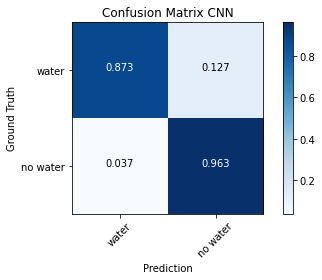
\includegraphics[width=\textwidth]{content/img/confusion_cnn.png}
        \caption{CNN}
    \end{subfigure}
    \begin{subfigure}{0.4\textwidth}
        \centering
        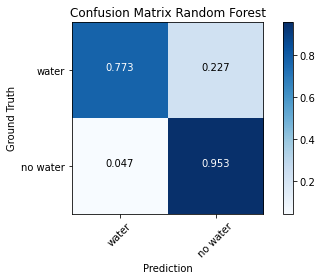
\includegraphics[width=\textwidth]{content/img/confusion_forest.png}
        \caption{Random Forest}
    \end{subfigure}
    \caption{Die Konfusionsmatrix für das Convolutional Neural Network (CNN) und für den Random Forest.}
    \label{fig:confusion}
\end{figure}
\begin{figure}
    \centering
    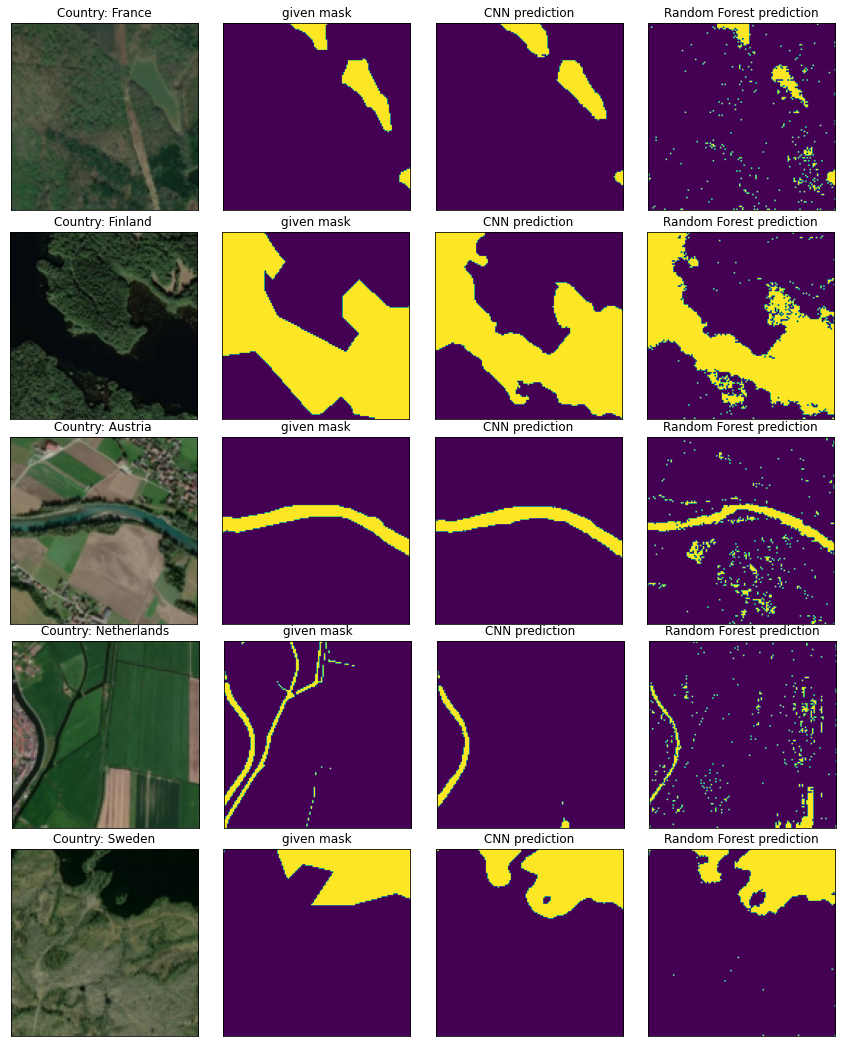
\includegraphics[width=\textwidth]{content/img/ergebnisse_bilder.png}
    \caption{Zufällige gezogene Ergebnisse des CNNs und Random Forest auf den Testdaten. \copyright Mapbox, \copyright OpenStreetMap}
    \label{fig:ergebnisse_bilder}
\end{figure}
Die Konfusionsmatrix in \autoref{fig:confusion} zeigt, dass Wasser zu $\SI{12.7}{\percent}$ (CNN) bzw. $\SI{22.7}{\percent}$ (Random Forest) fälschlicher Weise als 'kein Wasser' klassifiziert wird.
Hingegen wird 'kein Wasser' gerade mal zu $\SI{3.7}{\percent}$ für das tiefe Neuronale Netz und zu $\SI{4.7}{\percent}$ für den Random Forest als Wasser erkannt.
Das liegt unter anderem an der ungleichen Verteilung von Wasser und 'kein Wasser'.
Es sind ca. $\SI{33}{\percent}$ Wasserflächen auf den Satelliten- und Maskenbildern enthalten.
\\
\\
Insgesamt schneidet das Convolutional Neural Network sehr gut ab.
Zu beachten ist, dass die Satellitenbilder in einer geringen Auflösung vorliegen und dadurch wenige Details über die Gewässer bekannt sind.
Trotzdem konnte mit einer Genauigkeit von über $\SI{93}{\percent}$ Gewässer segmentiert werden.